\chapter{Introduction}
\label{cha:introduction}

The research work that I describe in this dissertation is concerned with the implementation of a Java framework, named \texttt{xmlet}, which allows the automatic generation of a Java \texttt{fluent interface}\cite{fluentinterface} recreating a \ac{DSL}\cite{dsl} described on a \ac{XML} schema. The approach described in this work can be further applied to any other strongly typed environment. As an example of \ac{DSL} generation we used \texttt{xmlet} to automatically create a Java \ac{DSL} for \ac{HTML}5, named \textit{HtmlFlow}. A \ac{DSL} for \ac{HTML} can be used as a type safe template engine which results in an improvement on the numerous existing \textit{template engines}. In this case, \textit{HtmlFlow} is the most efficient template engine for Java in several benchmarks containing over ten other \textit{template engines} introducing performance gains ranging from being slightly better than the second one to being twice as fast as the second best solution.

\section{Domain Specific Languages}

\lstdefinestyle{dynamicviewsex}{
  moredelim=**[is][\color{green}]{@}{@}, 
  moredelim=**[is][\color{blue}]{|}{|},
}

In the programming world there are multiple well-know programming languages such as Java, C and C\#. These language were created with the objective of being abstract, in the sense that they don't compromise with any specific problem. Using this generalist languages is usually enough to solve most problems but in some specific situations solving problems using exclusively those languages is counter-productive. A good example of that counter-productivity is thinking about regular expressions. In the Martin Fowler \ac{DSL} book\cite{dslbook} we have the following regular expression as an example presented in Listing \ref{lst:regexexpression}:

\bigskip

\begin{minipage}{\linewidth}
\begin{lstlisting}[caption={Regular Expression Example}, label={lst:regexexpression}, style=dynamicviewsex]
|\d{3}-\d{3}-\d{4}|
\end{lstlisting}
\end{minipage} 

\noindent
By looking at the expression the programmer understands that it matches a String similar to \texttt{123-321-1234}. Even though the regular expression syntax might be hard to understand at first it becomes understandable after a while and it's easier to use and manipulate than implementing the same set of rules to verify a \texttt{String} using control instructions such as \texttt{if/else} and \texttt{String} operations. It also makes the communication easier when dealing with this concrete problem because there's a standard syntax with defined rules that are acknowledged by the members of the conversation. Regular expressions are only one of the many examples that show that creating an extra language to deal with a very specific problem simplifies it, other examples of \ac{DSL}s are languages such as \ac{SQL}\footnote{\href{https://www.techopedia.com/definition/1245/structured-query-language-sql}{SQL Definition}}, \texttt{Apache Ant}\footnote{\href{https://www.techopedia.com/definition/16219/apache-ant}{Apache Ant Definition}} or \texttt{make}\footnote{\href{https://www.techopedia.com/definition/16406/make}{Make Definition}}. The \ac{DSL}s can be divided in two types, external or internal. External \ac{DSL} are languages created without any affiliations to a concrete programming language, an example of that is the regular expressions \ac{DSL}, since it defines its syntax without dependencies. An internal \ac{DSL} on the other side is defined within a programming language, such as Java. An example of an internal \ac{DSL} is the JMock\footnote{\href{http://jmock.org/}{JMock}} which is a Java library that provides tools for test-driven development. Internal \ac{DSL}s can also be referred to as embedded \ac{DSL}s since they are embedded in the language that they are using to define themselves. Other term to internal \ac{DSL}s is \textit{fluent interfaces} which are identified by the way that the usage of said \ac{DSL} can be read fluently.

\noindent
In this research what we are going to do can be summed up as a conversion of a external \ac{DSL} into an internal \ac{DSL}. On one side we have a \ac{XSD} document. A \ac{XSD} document defines a set of elements, attributes and rules that together define their own language. This language is qualified as an external \ac{DSL} since it is defined in \ac{XML} which is a markup language that doesn't depend on any programming language. This work has the objective of using all the information present in the \ac{XSD} document and generating a Java \textit{fluent interface}, which is an internal \ac{DSL} since it will use the Java syntax to define the \ac{DSL}. 

\noindent
In our use-case, the \ac{HTML}5 language, what we will need to do is to generate the respective \textit{fluent interface}, based on the information parsed from the \ac{HTML}5 \ac{XSD} document. The result of this translation of \ac{XSD} to Java will be the automatic code generation of Java classes and interfaces that will reflect all the information present in the \ac{XSD} document. When we analyze the end result of this work, what we achieve is a Java interface to manipulate a \ac{DSL}, in this case \ac{HTML}, which can be used for anything related with \ac{HTML} manipulation with the upside of having the guarantee that the rules of that language are verified. One of those usages is writing well-formed \ac{HTML} documents and defining \textit{dynamic views} that will be filled with information received in run-time.

\section{Dynamic Views}

A \textit{dynamic view} is a type of textual document that defines a view to represent information. To represent the information the document has two distinct components, as shown in Listing \ref{lst:dynamicstudentinfo}, a {\color{blue}static component}, represented in blue, which defines the structure of the document and a {\color{green}dynamic component}, represented in green, which is represented by \textit{placeholders} which indicate where to place the received information. A simple example of a \textit{dynamic view} can be an \ac{HTML} page that presents the information of a given \texttt{Student} as shown in Listing \ref{lst:dynamicstudentinfo}. 

\bigskip

\begin{minipage}{\linewidth}
\begin{lstlisting}[caption={Dynamic Student Info - Using Mustache Template Engine}, label={lst:dynamicstudentinfo}, style=dynamicviewsex]
|<html>
    <body>
        <ul>|
        @{{#student}}
            <li>
                {{name}}
            </li>
            <li>
                {{number}}
            </li>
        {{/student}}@
|        </ul>
    </body>
</html>|
\end{lstlisting}
\end{minipage} 

\noindent
To generate a complete view using the previous example we need external input, received in runtime, to replace the dynamic aspect of the view. In the previous example, Listing \ref{lst:dynamicstudentinfo}, the view needs to receive a value for the variable named \texttt{\char`\{\char`\{student\char`\}\char`\}}. The type that the \texttt{student} variable represents should be a type that contains two fields, a \texttt{number} and a \texttt{name} field. An example of an object with that characteristics is presented in Figure \ref{img:studentclass}.

\begin{figure}[H]
	\centering
	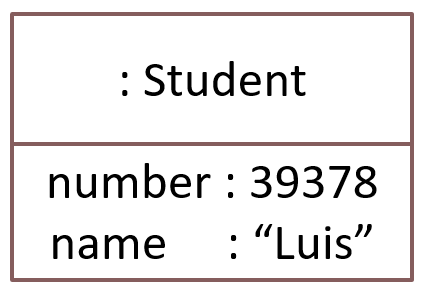
\includegraphics[width=0.35\textwidth]{student_class}
	\caption{Student Object}
	\label{img:studentclass}
\end{figure}

\noindent
Now that we have the two main ingredients for the proper construction of a \textit{dynamic view} we can see the \ac{HTML} document which results on the junction of these two aspects in Listing \ref{lst:dynamicstudentinfocomplete}.

\bigskip

\lstset{language=html}

\begin{minipage}{\linewidth}
\begin{lstlisting}[caption={Dynamic Student Info}, label={lst:dynamicstudentinfocomplete}]
<html>
    <body>
        <ul>
            <li>
                Luis
            </li>
            <li>
                39378
            </li>
        </ul>
    </body>
</html>
\end{lstlisting}
\end{minipage} 

\section{Template Engines}
\label{sec:templateengines}

The \textit{template engines} are the entity which is responsible for generating the \ac{HTML} document presented in Listing \ref{lst:dynamicstudentinfocomplete}. \textit{Template engines} are the most common method to manipulate \textit{dynamic views}. \textit{Template engines} are responsible for performing the combination between the \textit{dynamic view}, also named \textit{template}, and a data model, which contains all the information required to generate a complete document as shown in Figure \ref{img:templateengineprocess}.

\begin{figure}[H]
	\centering
	
\includegraphics[width=1\textwidth]{template_engines}
	\caption{Template Engine Process}
	\label{img:templateengineprocess}
\end{figure}

\noindent
Since the Web appearance to this day there is a wide consensus around the usage of \textit{template engines} to generate dynamic \ac{HTML} documents. The consensus is such that there isn't a real alternative to the usage of \textit{template engines} for dynamic generation of documents.  The \textit{template engine} scope is also wide, even that they are mostly associated with Web and its associated technologies they are also widely used to generate other types of documents such as emails and reports. 

\subsection{Template Engines Handicaps}
\label{sec:templateengineshandicaps}

Although there is a wide consensus in the usage of \textit{template engines} this type of solution still contain some handicaps, which we will further analyze.

\begin{itemize}
	\item Language Compilation - There is no compilation of the language used in the templates nor the dynamic information. This can result in documents that don't follow the language rules.
	\item Performance - This aspect can be divided in two, one regarding the text files that are used as templates which have to be loaded and therefore slow the overall performance of the application and the heavy usage of \texttt{String} operations which are inherently slow.
	\item Flexibility - The syntax provided by the \textit{template engines} is sometimes very limited which limits the operations that can be performed in the template files, often to if/else operations and the for operation to loop data.
	\item Complexity - It introduces more syntaxes to the programmer, for example a Java application using the Mustache\footnote{\href{https://mustache.github.io/}{Mustache Template Engine}} template engine to generate \ac{HTML} forces the programmer to use three distinct languages, Java, the Mustache syntax in the template file and the \ac{HTML} language.
\end{itemize}

\noindent
These are the main problems that exist within the \textit{template engines} solutions. To suppress these handicaps presented above we propose to use the solution implemented in this work, \texttt{xmlet}, which allows the automatic generation of a strongly typed and fluent interface for a \ac{DSL} based on the rules expressed in the \ac{XSD} document of that respective language, such as \ac{HTML}. How will the \texttt{xmlet} solution address the handicaps of the \textit{template engines}?

\begin{itemize}
	\item Language Compilation - The generated Java \ac{DSL} will guarantee the implementation of the language restrictions defined in the \ac{XSD} file by reflecting those restrictions to the Java language and enforce them by using the Java compiler.
	\item Performance - The text files to contain templates are replaced by Java functions that represent templates, removing the need to load an additional textual file.
	\item Flexibility - The syntax to perform operations on templates is changed to the Java syntax which is much more flexible than any template engine syntax.
	\item Complexity - It removes the requirement to write three distinct languages, the programmer only needs to program in Java.
\end{itemize}

\noindent
To understand how the generated \textit{fluent interface} will work we will present a little example, Listing \ref{lst:xmletdynamicstudentinfo}, that shows how the previous example in the Mustache idiom (Listing \ref{lst:dynamicstudentinfo}) will be recreated with the \texttt{xmlet} solution. The specific details on how the code presented in this example works will be provided in Chapter \ref{cha:solution}.

\bigskip

\lstset{language=java, morekeywords={String, DynamicHtml, view, render, CurrentClass, studentView, Student, html, body, ul, li, dynamic, text, getName, getNumber}}

\begin{minipage}{\linewidth}
\begin{lstlisting}[caption={Xmlet Dynamic Hello}, label={lst:xmletdynamicstudentinfo}, literate={º}{\textdegree}1]
String document = DynamicHtml.view(CurrentClass::studentView)
                             .render(new Student("Luis", 39378));

static void studentView(DynamicHtml<Student> view, Student student){
    view.html()
          .body()
            .ul()
              .li().dynamic(li -> li.text(student.getName())).º()
              .li().dynamic(li -> li.text(student.getNumber())).º()
            .º()
          .º()
        .º();   
}
\end{lstlisting}
\end{minipage} 

\section{Thesis statement}
\label{sec:thesisstatement}

This dissertation thesis is that it is possible to reduce the time spent by programmers by creating a process that automatizes the creation of \ac{DSL}s based on a preexisting \ac{DSL} defined in a \ac{XSD} document. The process encompasses three distinct aspects:

\begin{itemize}
	\item XsdParser - Which parses the \ac{DSL} described in a \ac{XSD} document in order to extract information needed to generate the internal Java \ac{DSL}.
	\item XsdAsm - Which uses XsdParser to gather the required information to generate the internal Java \ac{DSL}.
	\item HtmlApi - A concrete Java \ac{DSL} for the \ac{HTML}5 language generated by XsdAsm using the \ac{HTML}5 \ac{XSD} document.
\end{itemize}

\noindent
The use case used in this dissertation will be the \ac{HTML} language but the process is designed to support any domain language that has its definition in the \ac{XSD} syntax. This means that any \ac{XML} language should be supported as long as it has its set of rules properly defined in a \ac{XSD} file. To show that this solution is viable with other \ac{XSD} files we used another \ac{XSD} file that detailed the rules of the \ac{XML} syntax used to generated Android\footnote{\href{https://www.android.com/}{Android}} visual layouts.

\section{Document Organization}

This document will be separated in six distinct chapters. The first chapter, this one, introduces the concept that will be explored in this dissertation. The second chapter introduces the motivation for this dissertation. The third chapter presents existent technology that is relevant to this solution. The fourth chapter explains in detail the different components of the suggested solution. The fifth chapter approaches the deployment, testing and compares the \texttt{xmlet} solution to other existing solutions. The sixth and last chapter of this document contains some final remarks and description of future work.